\section{Auswertung}
\subsection{Wertetabelle}
\begin{table}[H]
    \centering
    \begin{tabular}{c | c c c c c}
        \toprule
        & Feder 1 & Feder 2 & Feder 3 & Feder 4 & Feder 5 \\ & (Basisfeder)\\
        \midrule
        $m\;/\;$g Stk. & 1.3456 & 1.311 & 1.3812 & 1.4574 & 1.2342 \\
        \midrule
        $D_a\;/\;$mm & 3.68 & 3.57 & 3.82 & 3.69 & 3.69 \\
          & 3.67 & 3.57 & 3.81 & 3.68 & 3.69 \\
          & 3.69 & 3.57 & 3.82 & 3.68 & 3.68 \\
          & 3.68 & 3.57 & 3.82 & 3.68 & 3.68 \\
          & 3.69 & 3.57 & 3.82 & 3.76 & 3.68 \\
          & 3.68 &         &         &         &         \\
        \midrule
        $\bar{D_a}\;/\;$mm & 3.68  & 3.57 & 3.818 & 3.69 & 3.684\\
        $D_{a_S}\;/\;$mm& 0.007 & 0 & 0.004 & 0.03 & 0.005\\
        \midrule
        $L0$ 	& 57.04 	& 57.3 		& 56.38 	& 61.15 	& 52.73 	\\
                & 57.17 	& 57.39 	& 56.69 	& 61.22 	& 52.81 	\\
                & 57.07 	& 57.27 	& 56.6 		& 61.31 	& 52.86 	\\
                & 57.16 	& 57.41 	& 56.66 	& 61.29 	& 52.97 	\\
                & 56.89 	& 57.27 	& 56.89 	& 61.2 		& 52.82 	\\
                & 57.04 	&         	&         	&         	&   \\
        \midrule
        $\bar{L0}\;/\;$mm & 57.06 	& 57.33 	& 56.64 	& 61.23 	& 52.84	\\
        $L0{_S}\;/\;$mm & 0.093 	& 0.060 	& 0.16 	& 0.059 	& 0.078	\\
        $n_{wirk}$ & 109.36 & 109.98 & 108.39 & 119.07 & 99.54 \\(berechnet)\\
        \midrule
        $F1\;/\;$N bei $L1=105\;$mm & 4.8 & 5.21 & 4.46 & 4.26 & 5.5\\
                         & 4.86 & 5.28 & 4.48 & 4.25 & 5.5\\
                         & 4.83 & 5.29 & 4.5 & 4.3 & 5.48\\
                         & 4.83 & 5.28 & 4.49 & 4.28 & 5.47\\
                         & 4.85 & 5.29 & 4.52 & 4.23 & 5.49\\
        \midrule
        $F2\;/\;$N bei $L2=142\;$mm & 7.97 & 8.7 & 7.33 & 7.2 & 8.93\\
                         & 8.02 & 8.75 & 7.33 & 7.17 & 8.92\\
                         & 7.96 & 8.73 & 7.35 & 7.22 & 8.93\\
                         & 8.0 & 8.75 & 7.35 & 7.2 & 8.9\\
                         & 8.04 & 8.77 & 7.4 & 7.14 & 8.93\\
        \midrule
        $\bar{F1}\;/\;$N & 4.83 & 5.27 & 4.49 & 4.264 & 5.49\\
        $F1_S\;/\;N$     & 0.021& 0.03 & 0.02 & 0.0241& 0.012\\ 
        $\bar{F2}\;/\;$N & 7.99 & 8.74 & 7.35 & 7.19 & 8.92\\
        $F2_S\;/\;N$     & 0.03 &0.024 & 0.026& 0.028& 0.017\\ 
        \midrule
        $R $ & 0.086 & 0.094 & 0.077 & 0.079 & 0.093\\
        \midrule
        $F_0\;/\;$N & 0.73 & 0.79 & 0.75 & 0.81 & 0.65\\ 
        \bottomrule
    \end{tabular}
    \caption{$m$ Federmasse,
             $D_a$ Federaußendruchmesser, 
             $\bar{D_a}$ Mittelwert des Federaußendruchmesser, 
             $D_{a_S}$ Standartabweichung des Federaußendruchmesser,
             $L_0$ Federlänge,
             $\bar{L}$ Mittelwert der Federlänge,
             $L_{0_S}$ Standartabweichung der Federlänge,
             $n_{wirk}$ wirkende Windungszahl,
             $F1$,$F2$ Federkräfte,
             $\bar{F1}$,$\bar{F2}$ Mittelwert der Federkräfte,
             $R$ Federkonstante,
             $F0$ Innere Vorspannkraft
    }
    \label{tab:Wertetabelle}
\end{table}


\subsection{Variable Federdicke}
\label{sec:federdicke}
Im Folgenden werden die wirkenden Windung $n_{wirk}$ als konstant mit $n_1=109.4$ angenommen, 
da die maximale Abweichung von $\Delta n_{max}=0.97$, resultierend aus nicht beeinflussbaren
Fertigungsprozessen, als hinreichend klein angenommen wird.


\begin{figure}[H]
    \center
    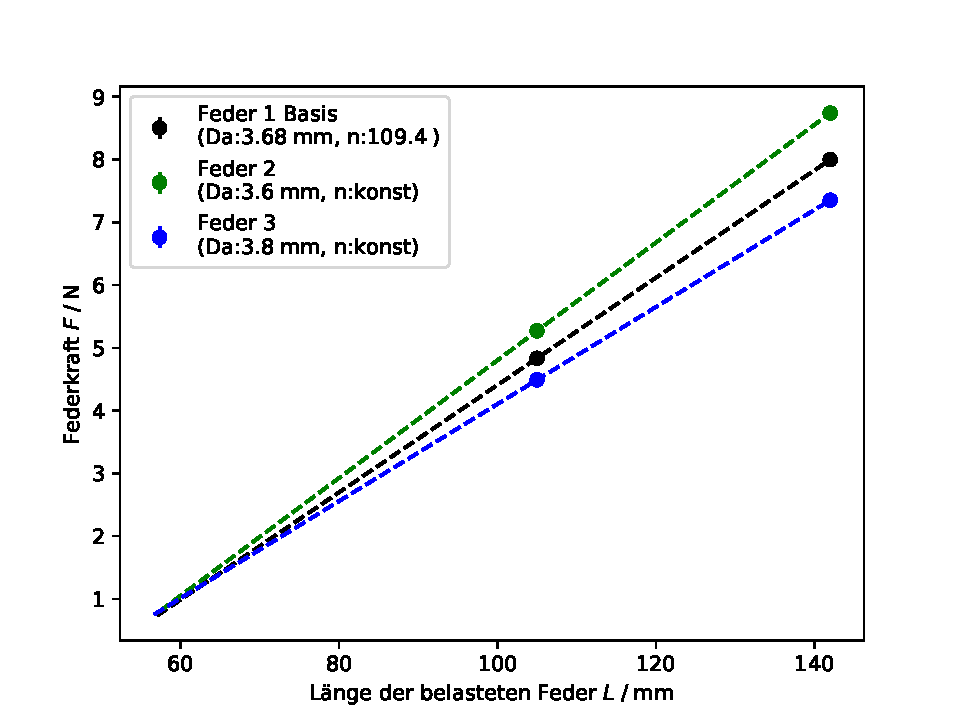
\includegraphics[width=0.8\textwidth]{plots/D_kraftweg_dia.pdf}
    \caption{Feder 1,2,3 mit unterschiedlichen Federaußendurchmessern $D_a$ bei konstanter Basiswindungszahl $n$.
    Aufgetragen in einem Kraft-Weg-Diagramm. Gemessen wurden dabei
    die für L1 und L2 resultierenden Federkräfte F1 und F2.}
    \label{tab:LF_D}
\end{figure}
\subsubsection{Lineare Ausgleichsgerade}
\label{sec:fit}
Für die jeweiligen Ausgleichsgeraden aus \ref{tab:LF_D} wird ein Polyfit \cite{numpy_polyfit}
ersten Grades durchgeführt und daraus die Steigung, also die Federkonstante $R$ so wie eine Verschiebung
in der vertikalen $v$ ermittelt.\\
Aus \ref{eqn:federrate} mit
\begin{align*}
  F&=R \cdot L + v ,\\
  F&=R \cdot s + F0,
\end{align*}
folgen somit die in \ref{tab:Wertetabelle} aufgeführten Federkonstanten.
\begin{align*}
  R1= 0.086\;\si{\N\per\mm}, &&  v1= -4.14\;\si{\N},\\
  R2= 0.094\;\si{\N\per\mm}, &&  v2= -4.58\;\si{\N},\\
  R3= 0.077\;\si{\N\per\mm}, &&  v3= -3.63\;\si{\N}.\\
\end{align*}

\subsubsection{Innere Vorspannkraft ermitteln}
\label{sec:vorspannkraft}
Von dem Verschiebungswerten $v$ schließe man auf die innere Vorspannkraft $F_0$ durch das Verschieben
der Gerade, sodass nun der Federweg $s$ betrachtet wird.
\begin{align*}
  F&=R \cdot L + v\\
  F&=R \cdot s + (v+L0 \cdot R) \text{ mit }F0:= (v+L0 \cdot R) \\
\end{align*}
\begin{figure}[H]
  \center
  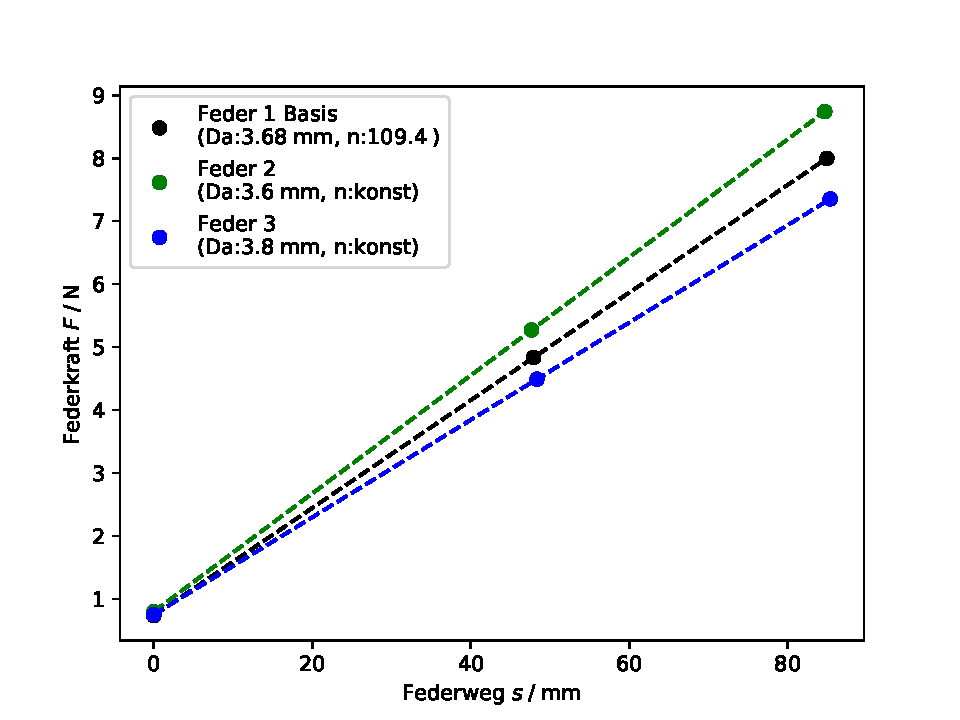
\includegraphics[width=0.8\textwidth]{plots/f0_123_dia.pdf}
  \caption
  {
    Federkraft $F$ betrachtet für Federweg $s$, y-Achsenabschnittet bildet dabei die innere Vorspannkraft $F_0$.
    So folgt aus einer Geradengleichung mit $y_0=R\cdot(L-L_0)+b$ dass $y_{\Delta L}=y_0+R \cdot L_0=R \cdot L+b$
    wobei für $L=0$ folglich gilt $y_{\Delta L}(L=0)=b=:F_0$.
  }
\end{figure}
Somit ergeben sich für die jeweilligen inneren Vorspannkräfte $F0$
\begin{align*}
  F0_1=  0.73 \;\si{\N},\\
  F0_2=  0.79 \;\si{\N},\\
  F0_3=  0.75 \;\si{\N}.\\
\end{align*}


\subsubsection{Einfluss auf die Federkonstante}

\begin{figure}[H]
  \center
  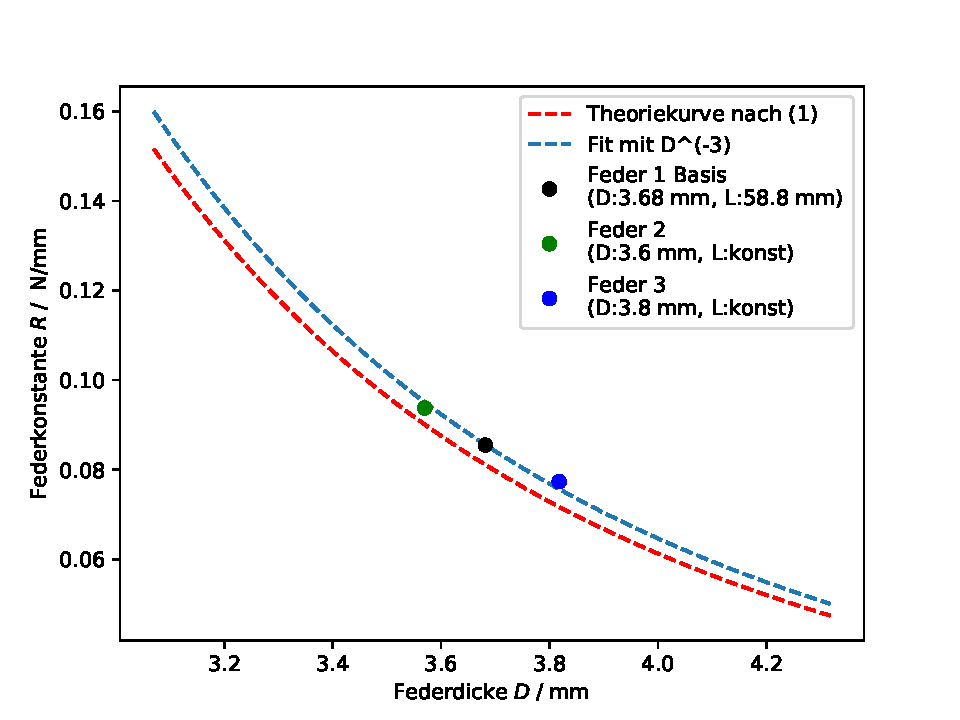
\includegraphics[width=0.8\textwidth]{plots/dicke_konstante_dia.pdf}
  \caption{Die Federdicke $D_a$ gegen die Federkonstante $R$ aufgetragen.}
  \label{fig:R_D_dia}
\end{figure}

Es folgt für die Ausgleichsgerade aus \ref{eqn:federrate}
\begin{align*}
  R=\frac{G\;d^4}{8\;n}\cdot \frac{1}{D^3}, \\\\  
  \text{mit }k_D =\frac{G\;d^4}{8\;n}.
\end{align*}
Es folgt die Funktion
\begin{equation*}
  R(D)=k_D \cdot \frac{1}{D^3},
\end{equation*}
mit dem Parameter
\begin{equation*}
  k_D=(2.94 \pm 0.03) \;\si{\N\mm\squared}
\end{equation*}


\subsection{Variable Federwindungszahl}
\label{sec:federwindungen}
\begin{figure}[H]
    \center
    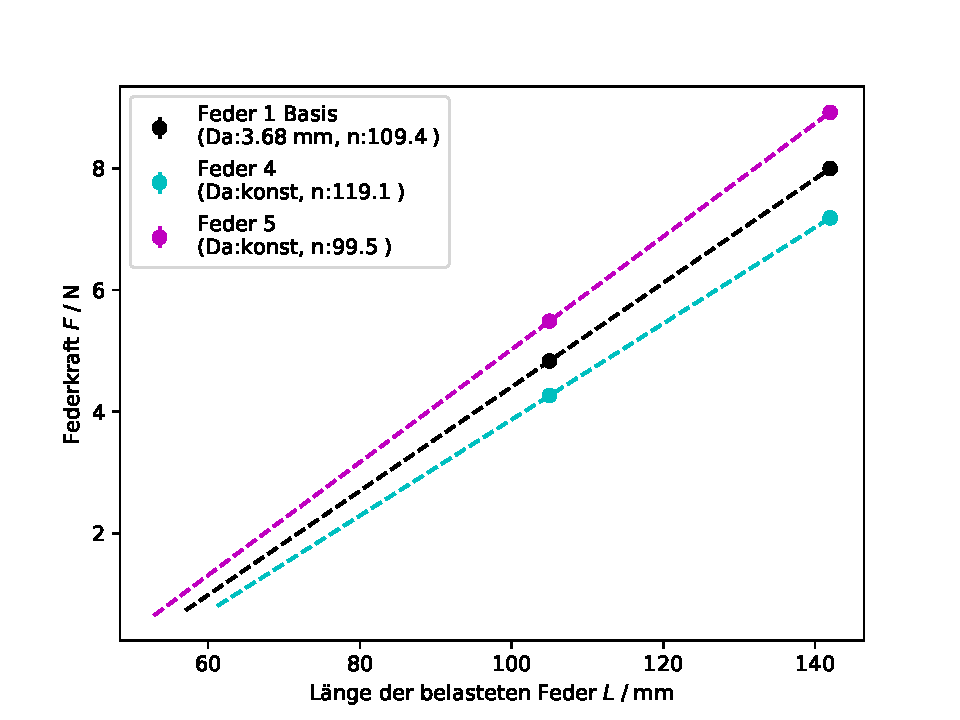
\includegraphics[width=0.8\textwidth]{plots/n_kraftweg_dia.pdf}
    \caption{Feder 1,4,5 mit unterschiedlichen Windungszahlen $n$ bei konstanter Basis Federdicke $D_a$.
    Aufgetragen in einem Kraft-Weg-Diagramm. Gemessen wurden dabei die für L1
    und L2 resultierenden Federkräfte F1 und F2}
\end{figure}

\subsubsection{Federkonstante und Innere Vorspannkraft}
Analog wie in Abschnitt \ref{sec:fit} folgt für die Federkonstante $R$
und den Verschiebungswert $v$, aus dem, mit der Methodik \ref{sec:vorspannkraft},
die innere Vorspannkraft $F_0$ ermittelt wird
\begin{align*}
  R1= 0.086\;\si{\N\per\mm}, &&  v1= -4.14\;\si{\N}, && F0_1=0.73\;\si{\N}\\
  R4= 0.079\;\si{\N\per\mm}, &&  v4= -4.03\;\si{\N}, && F0_4=0.81\;\si{\N}\\
  R5= 0.092\;\si{\N\per\mm}, &&  v5= -4.26\;\si{\N}. && F0_5=0.65\;\si{\N}\\
\end{align*}


\subsubsection{Einfluss auf die Federkonstante}
\begin{figure}[H]
  \center
  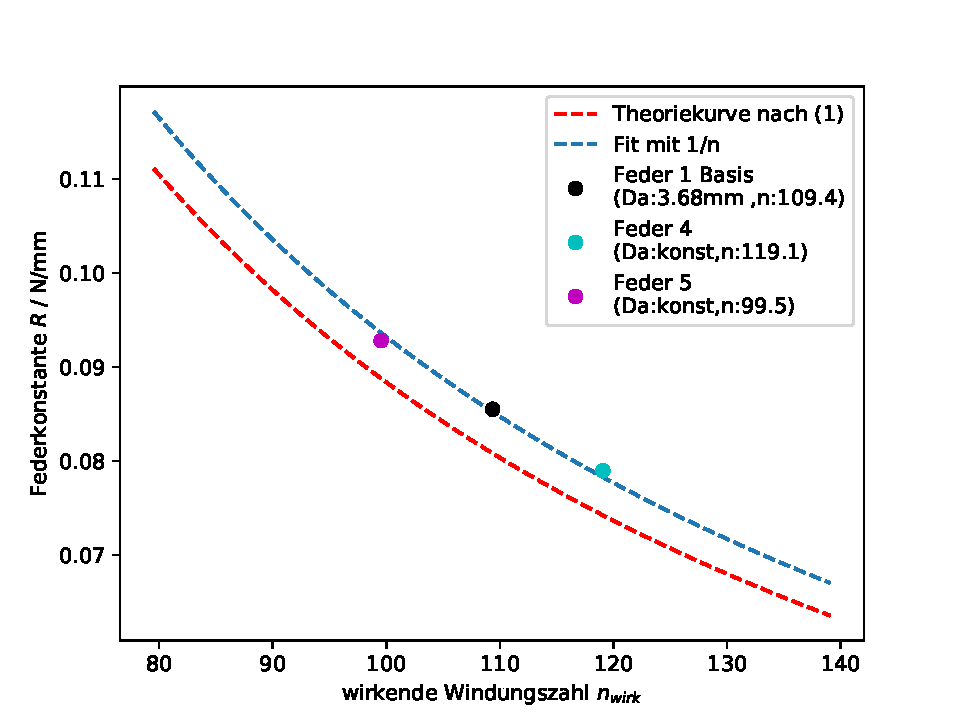
\includegraphics[width=0.8\textwidth]{plots/n_konstante_dia.pdf}
  \caption{Einfluss der Windungszahl $n_{wirk}$ auf die Federkonstante $R$}
  \label{fig:R_n_dia}
\end{figure}
Es folgt für die Ausgleichsgerade aus \ref{eqn:federrate}
\begin{align*}
  R=\frac{G\;d^4}{8\;D^3}\cdot \frac{1}{n_{wirk}} \\\\  
  \text{mit } k_n=\frac{G\;d^4}{8\;D^3}
\end{align*}
Es folgt die Funktion
\begin{equation*}
  R(n)=k_n \cdot \frac{1}{n_{wirk}}
\end{equation*}
mit dem Parameter
\begin{equation*}
  k_n=(9.32 \pm 0.05) \;\si{\N\per\mm}
\end{equation*}


\subsection{Betrachtung der Masse}
\begin{figure}[H]
  \center
  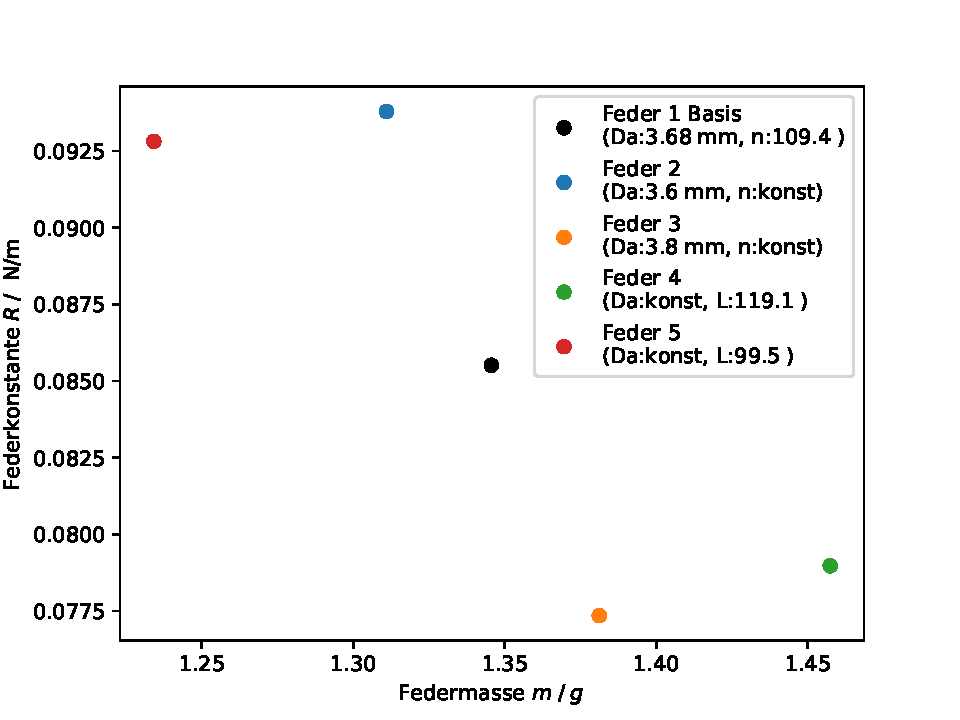
\includegraphics[width=0.8\textwidth]{plots/masse_konstante_dia.pdf}
  \caption{Massenresulate aus der Variation der Federdicke $D_a$
          und der Windungszahl $n$ der Federkonstanten $R$ gegenübergestellt. }
\end{figure}
Mit der hergeleiteten Formel \ref{eqn:masse} für die Masse in Abhängigkeit von dem Federdurchmesser und der Windungszahl lassen sich die beiden Abhängigkeiten graphisch darstellen und eine Ausgleichsrechnung durchführen.
Bei der Ausgleichsrechnung fällt auf, dass sie sich im gegebenen Intervall annähernd linear verhält. 
Somit kann der Einfluss der beiden Größen anhand der linearen Ausgleichsrechnung 
abgeschätzt werden.
\begin{figure}[H]
  \center
  \includegraphics[width=0.8\textwidth]{plots/Masse_D.pdf}
  \caption{}
\end{figure}
\begin{figure}[H]
  \center
  \includegraphics[width=0.8\textwidth]{plots/Masse_n.pdf}
  \caption{}
\end{figure}
Durch die Lineare Regression ergibt sich für den Durchmesser $D$ eine Steigung von $m = 0,282\pm0,016$ und für die Windungszahl $n$ eine Steigung von $m = 0,0113\pm0,0027$.
\label{sec:Auswertung}
